% !TeX root = main.tex
\section*{Results and discussion}
\begin{figure*}[!t]
    \centering
    \begin{subfigure}[t]{0.24\linewidth}
    	\centering
    	\resizebox{\linewidth}{!}{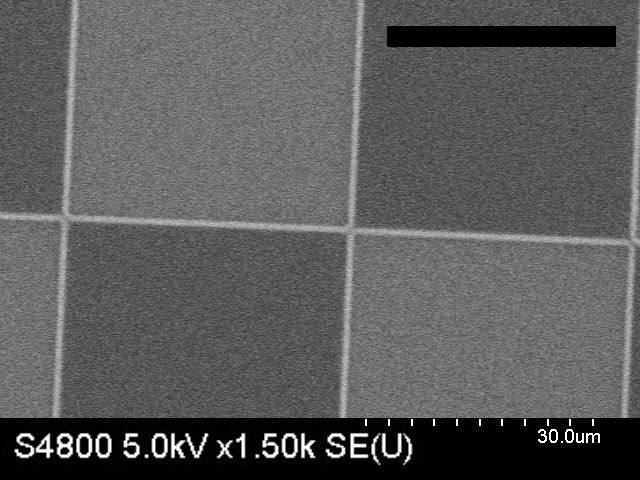
\includegraphics{data/sem/b3a5_q05.jpg}}
    	\caption{Largest checkerboard. Black scale bar is 30.0~$\mu$m wide.}
    	\label{fig:b2d5_q5}
    \end{subfigure}
    \hfill
    \begin{subfigure}[t]{0.24\linewidth}
    	\centering
    	\resizebox{\linewidth}{!}{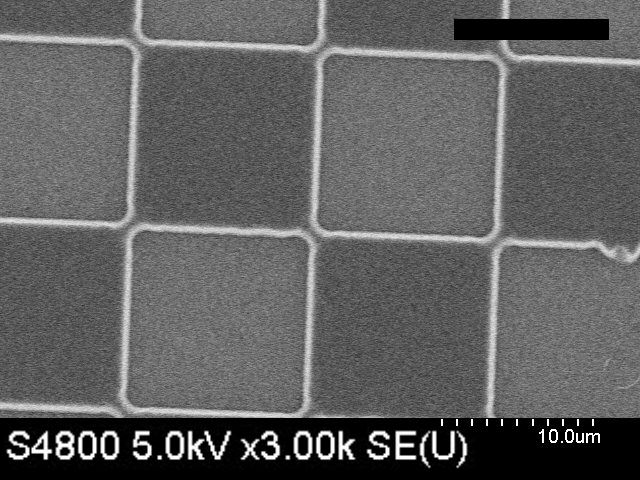
\includegraphics{data/sem/b3a7_q07.jpg}}
    	\caption{Slight overexposure can be seen at the vertices of the squares. Black scale bar is 10.0~$\mu$m wide.}
    	\label{fig:b2d7_q7}
    \end{subfigure}
    \hfill
    \begin{subfigure}[t]{0.24\linewidth}
    	\centering
    	\resizebox{\linewidth}{!}{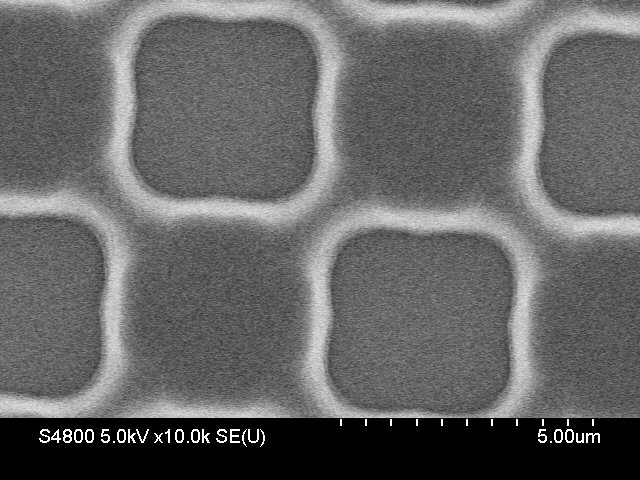
\includegraphics{data/sem/b3a9_q09.jpg}}
    	\caption{The effects of overexposure become pronounced here. Black scale bar is 5.00~$\mu$m wide.}
    	\label{fig:b2d9_q9}
    \end{subfigure}
    \hfill
    \begin{subfigure}[t]{0.24\linewidth}
    	\centering
    	\resizebox{\linewidth}{!}{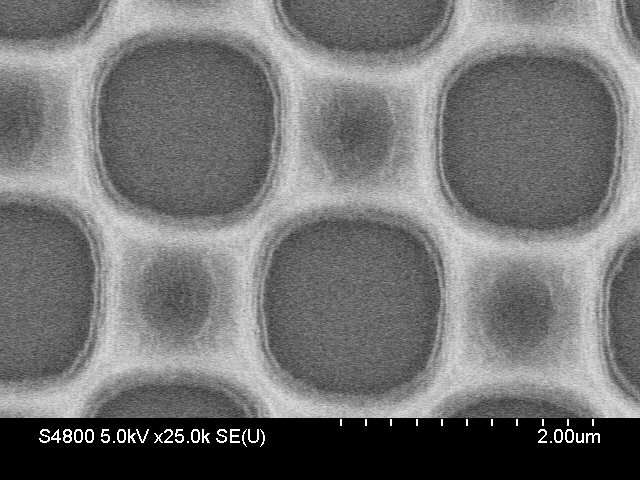
\includegraphics{data/sem/b3a10_q11.jpg}}
    	\caption{The patterns starts become unrecognizable. Black scale bar is 2.00~$\mu$m wide.}
    	\label{fig:b2d10_q11}
    \end{subfigure}
    \caption{SEM images of the checkerboard patterns in order of decreasing size on the positive tone sample. $\tau = 2$~min.}
\end{figure*}
\begin{figure*}[!b]
    \centering
    \begin{subfigure}[t]{0.3\linewidth}
        \centering
        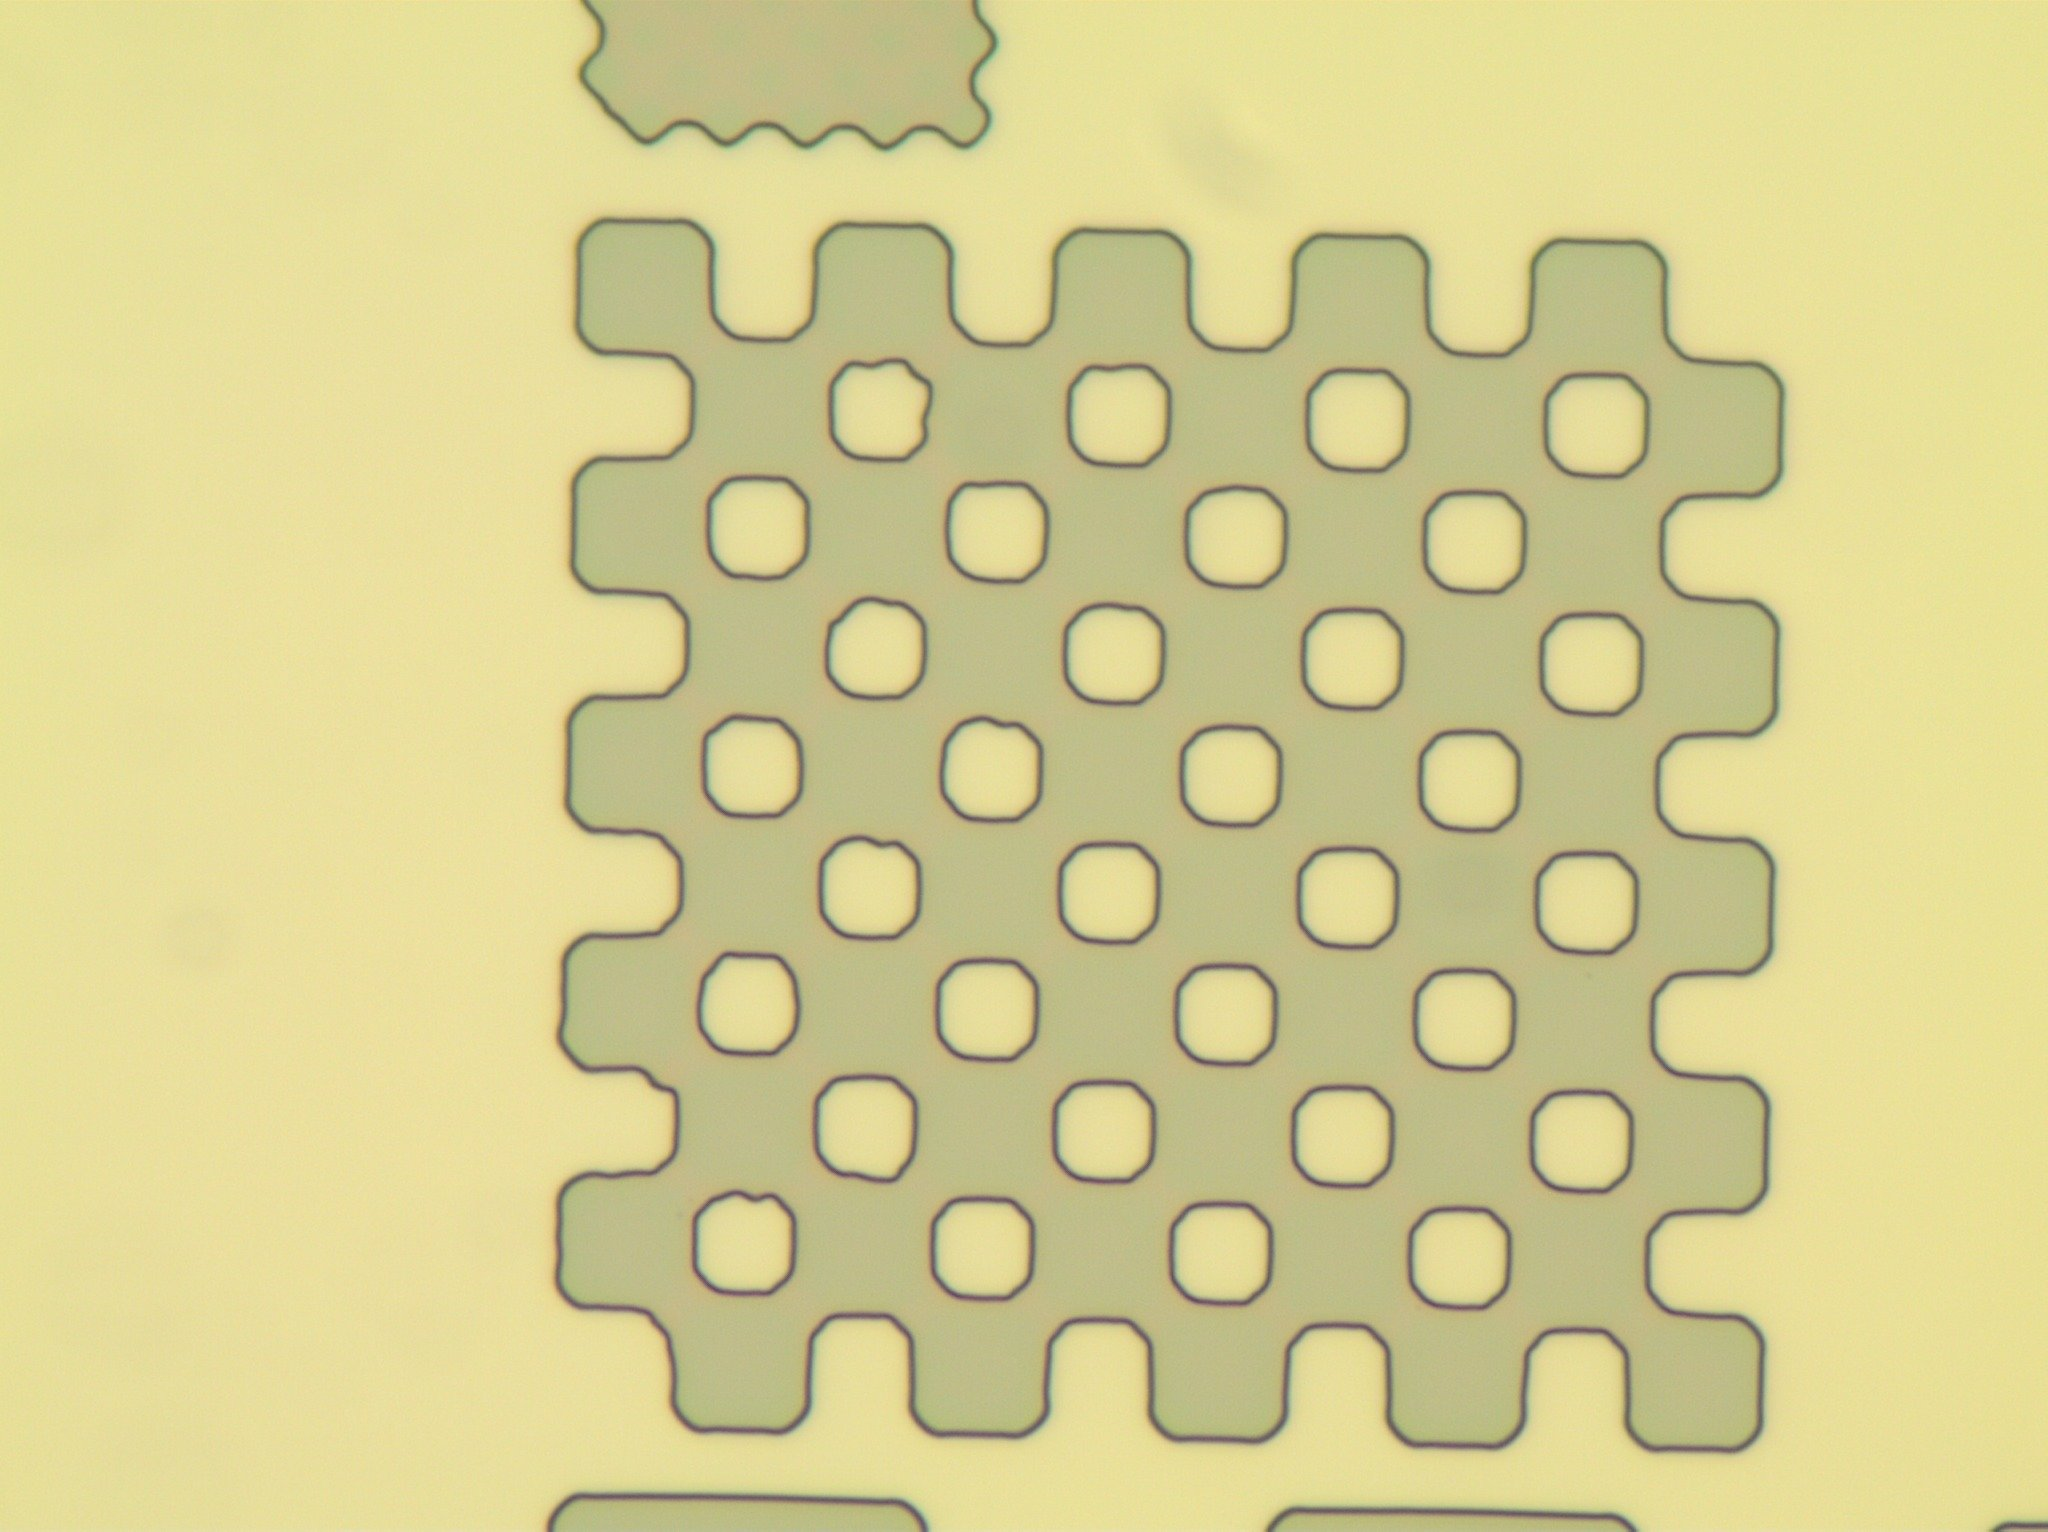
\includegraphics[width=\textwidth]{data/b2d1.jpg}
	    \caption{$\tau_1 = 0.5$~min. and $\tau_2 = 4$~min. Too much resist is cross-linked (grey areas) as a result of overexposure.}
	    \label{fig:b2d1}
    \end{subfigure}
    \hfill
    \begin{subfigure}[t]{0.3\linewidth}
        \centering
        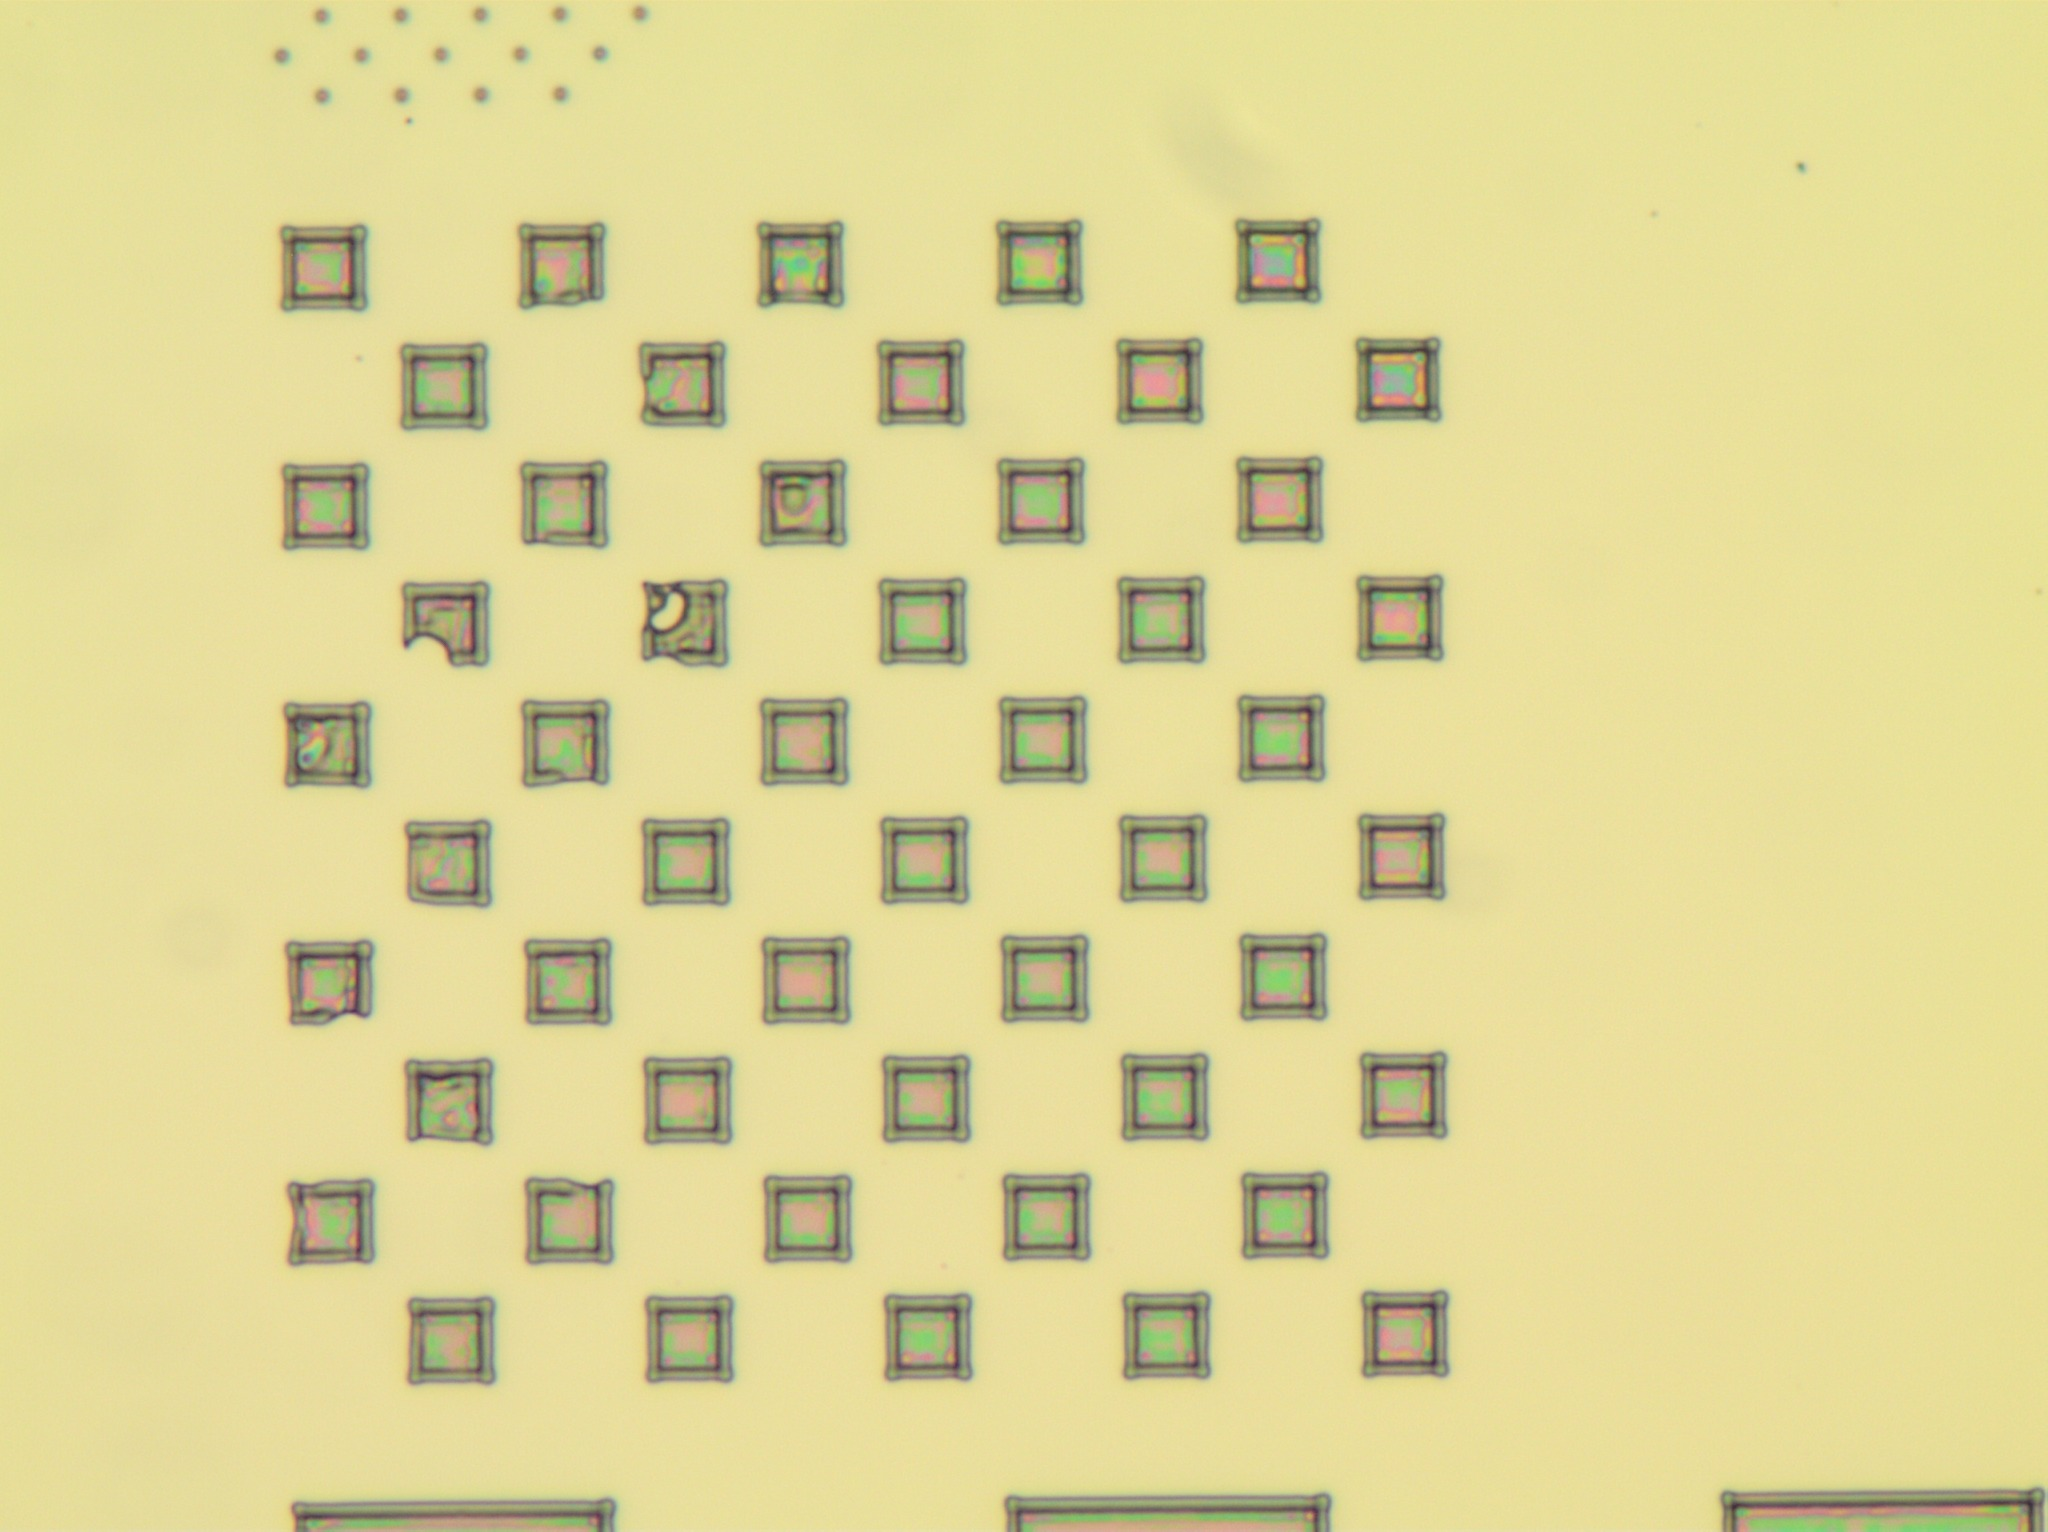
\includegraphics[width=\textwidth]{data/b2h1.jpg}
	    \caption{$\tau_1 = 0.2$~min. and $\tau_2 = 4$~min. Too little resist is cross-linked as a result of underexposure.}
	    \label{fig:b2h1}
    \end{subfigure}
    \hfill
    \begin{subfigure}[t]{0.3\linewidth}
        \centering
        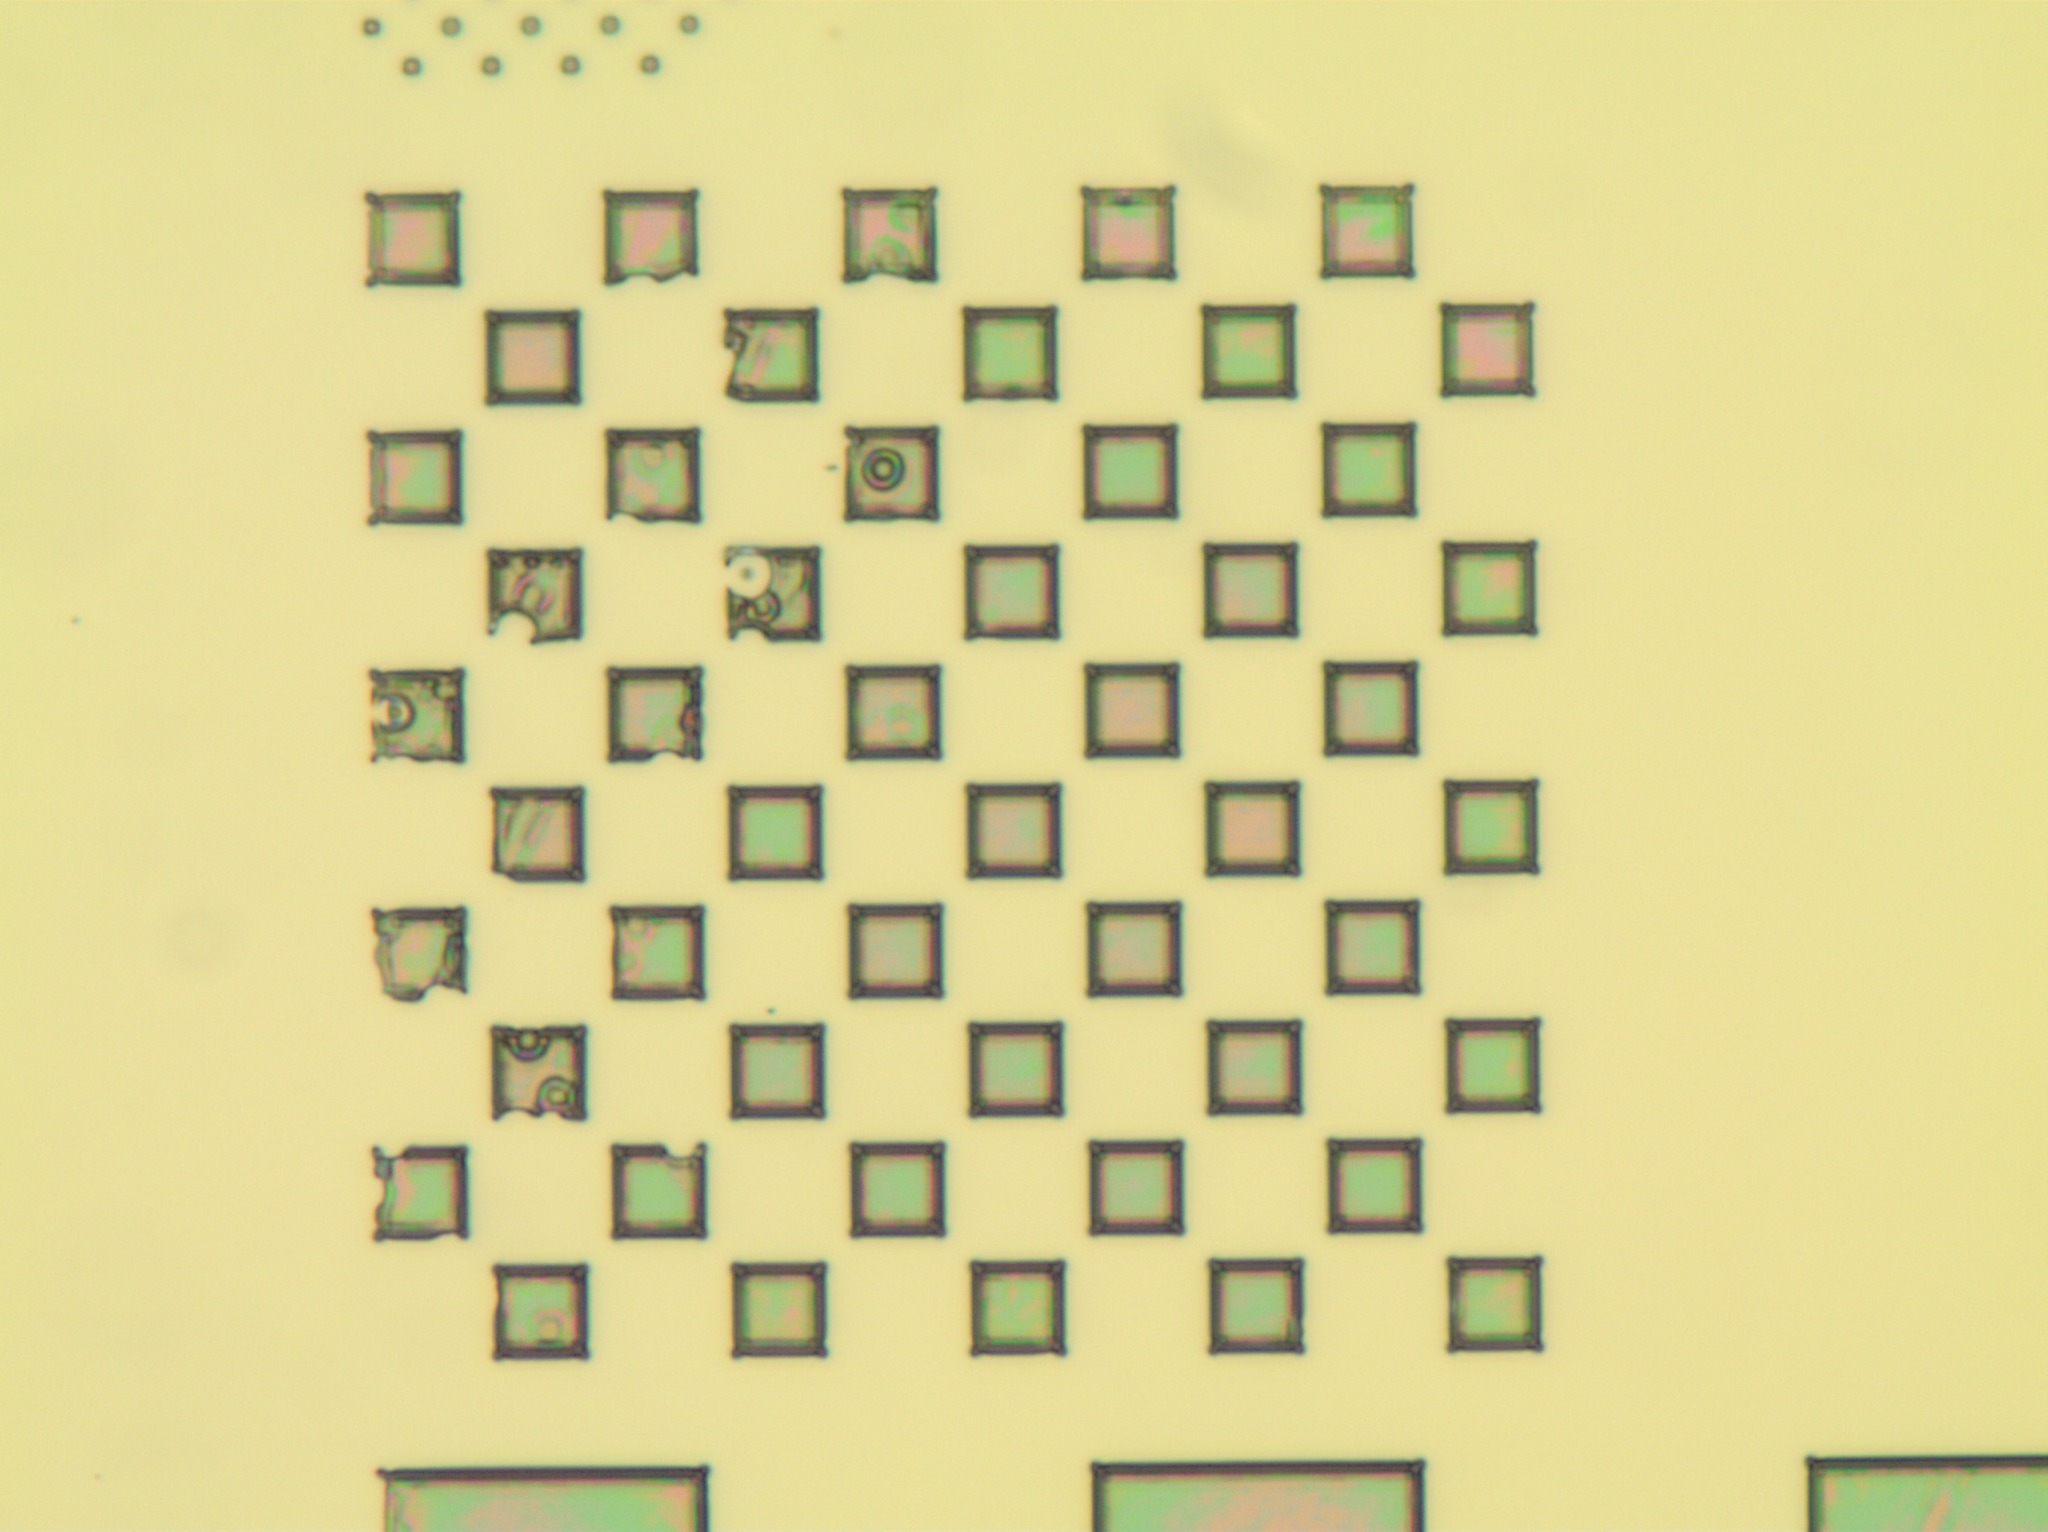
\includegraphics[width=\textwidth]{data/b2i1.jpg}
	    \caption{$\tau_1 = 0.3$~min. and $\tau_2 = 4$~min. The sample is again underexposed, but not as much as in subfigure \subref{fig:b2h1}.}
	    \label{fig:b2i1}
    \end{subfigure}
    \caption{Optical microscope images of the third largest checkerboard on the negative tone resist with different exposure times.}
    \label{fig:optical-neg}
\end{figure*}

\begin{figure*}[!t]
    \begin{subfigure}[t]{0.24\linewidth}
    	\centering
    	\resizebox{\linewidth}{!}{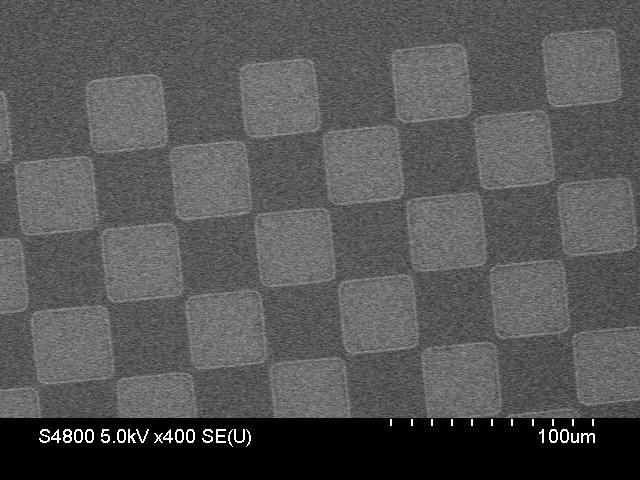
\includegraphics{data/sem/b2d26_q26.jpg}}
    	\caption{Largest checkerboard. Scale bar is 100~$\mu$m}
    	\label{fig:b2d26_q26}
    \end{subfigure}
    \hfill
    \begin{subfigure}[t]{0.24\linewidth}
    	\centering
    	\resizebox{\linewidth}{!}{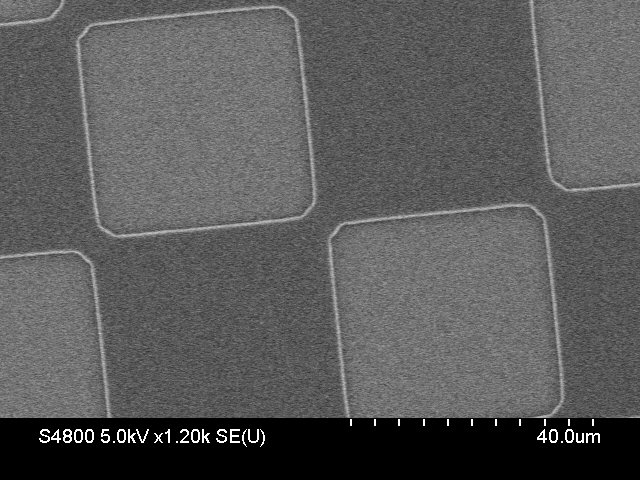
\includegraphics{data/sem/b2d27_q27.jpg}}
    	\caption{Largest checkerboard. Scale bar is 40~$\mu$m}
    	\label{fig:b2d27_q27}
    \end{subfigure}
    \hfill
    \begin{subfigure}[t]{0.24\linewidth}
    	\centering
    	\resizebox{\linewidth}{!}{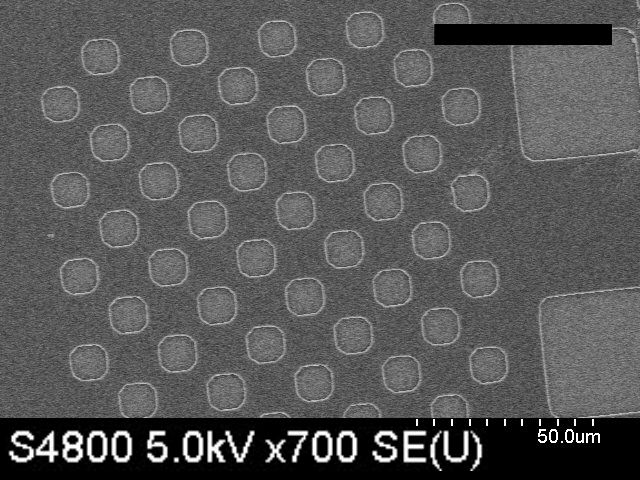
\includegraphics{data/sem/b2d28_q28.jpg}}
    	\caption{Second largest checkerboard. Scale bar is 50~$\mu$m}
    	\label{fig:b2d28_q28}
    \end{subfigure}
    \hfill
    \begin{subfigure}[t]{0.24\linewidth}
    	\centering
    	\resizebox{\linewidth}{!}{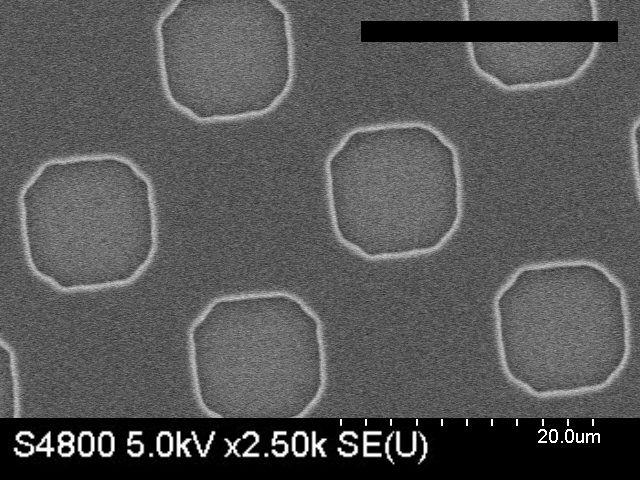
\includegraphics{data/sem/b2d29_q29.jpg}}
    	\caption{Second largest checkerboard. Scale bar is 20~$\mu$m}
    	\label{fig:b2d29_q29}
    \end{subfigure}
    \caption{SEM images of the two largest checkerboard patterns on the negative tone sample (inverse version of the patterns shown in figure \ref{fig:optical-neg}). $\tau_1 = 0.5$~min, $\tau_2 = 4$~min.}
    \label{fig:negative-sem}
\end{figure*}
The mask was made with a variety of shapes in different sizes, including but not limited to, checkerboards, outward radiating lines and shapes with optical proximity correction (OPC). The complete design is shown in figure \ref{fig:litho_design}. In this section only the checkerboard shapes are discussed as the other shapes did not contribute to more insight. A more complete overview of microscope images of the designed shapes can be found in appendix \ref{ap:inspec_img}.

To find the optimal exposure time $\tau$, the checkerboard pattern of each sample is inspected under an optical microscope. With a positive tone resist, underexposure results in not enough resist being dissolved in the development solution (figure \ref{fig:b3d1}). Of the exposed areas, the molecules near the boundary do not reach the dose threshold, while the molecules in the center do. This is because the molecules in the center receive much scattered light from neighbouring molecules, molecules near the boundary do not nearly have as many neighbours. When the resist is exposed for too long, boundary areas underneath the opaque parts of the mask also reach the dose threshold (figure \ref{fig:b3a1}). With the limited amount of developed samples, an exposure time of 2 minutes was found to be optimal (figure \ref{fig:b3e1}).

Images of the checkerboard patterns on the positive tone sample with an exposure time of 2 minutes were taken with a Hitachi S4800 scanning electron microscope. On the largest checkerboard (figure \ref{fig:b2d5_q5}) the exposure time appears to be just right. When looking at the smaller checkerboards however, the effects of overexposure become apparent (figure \ref{fig:b2d7_q7}-\subref{fig:b2d10_q11}). The bright areas around the pattern boundaries is due to the ``edge effect'', which is a result of more secondary electrons leaving the sample at the edges.

The negative tone has two exposure times that are varied, the initial exposure $\tau_1$ for the cross-linking and the flood exposure $\tau_2$. The first three samples were done with $\tau_2 = 3$~minutes. During the analysis of these samples it was found that the quality of the samples fluctuated, and that longer exposure times were required, thus $\tau_2 = 4$~minutes was used for the remaining samples.

It was found that for the negative tone resist an exposure time of 0.1 min. resulted in no pattern creation at all, while exposure times of 0.5 minutes and longer resulted in overexposure (figure \ref{fig:b2d1}). While an exposure time of 0.2 or 0.3 min. resulted in underexposure (figure \ref{fig:b2h1} and \subref{fig:b2i1} respectively). Thus an exposure time of around 0.4 minutes probably would have been optimal, but was not done due to lack of time. The negative tone sample where $\tau = 0.5$~min. was inspected in the SEM (figure \ref{fig:negative-sem}). The mask appeared to contain the pattern as designed and an inverse version. As a result, the SEM image are from the inverted design as opossed to the optical microscope images (figure \ref{fig:optical-neg}). From at the largest checkerboard (figure \ref{fig:b2d26_q26} and \subref{fig:b2d27_q27}) the overexposure is already apparent and becomes even more pronounced at the second and third largest checkerboards (figure \ref{fig:b2d28_q28} and \subref{fig:b2d29_q29}). The squares of the smaller versions have merged together to a single square.  \todo[inline]{What is that rainbow effect in figure \ref{fig:optical-neg}?}


% ================== Daniel checked up to here ===============

\todo[inline]{Where do the shadows in the optical images come from?}
The thickness of the resist layers is analyzed using a profilometer. A straight line was traced such that the probe scanned both exposed areas as well as  unexposed areas. The difference in height between the removed and untouched resist $\Delta h$ was determined from two scans at different locations on a sample. From table \ref{tab:pos_profile} it is clear that $\tau = 1$~min. is too short to completly remove the resist. From the longer exposure times, the thickness of the resist was measured at around 1.6~$\mu$m, which is thicker than the expected 1.4~$\mu$m for AZ~5214~E at 4000~rpm.
\begin{table}[H]
    \centering
    \caption{Positive tone resist height difference between exposed and unexposed areas.}
    \begin{tabular}{X l l l}
        $\tau$ (min)& $\Delta h$ ($\mu$m) \\
        \hline\hline
        1.0 & 0.3175(3) \\
        2.5 & 1.6286(4) \\
        3.0 & 1.5932(2) \\
        3.5 & 1.5920(3) \\
        4.0 & 1.6696(3) \\
        \hline
    \end{tabular}
    \label{tab:pos_profile}
\end{table} For the negative samples (table \ref{tab:neg_profile}) $\tau_1 \leq 0.3$~min. is too short for the cross-linking to reach the full height of the resist. For $\tau_1 = 0.1$~min. no patterns were visible at all and no significant height difference was measured. The height difference for longer $\tau_1$ is smaller than for the positive resist, although still larger than expected. A possible explanation is that some part of the primer is also removed during development, creating a larger height difference. \todo[inline]{Does this make sense ???}
\begin{table}[H]
    \centering
    \caption{Negative tone resist height difference between cross-linked and areas without cross-links.}
    \begin{tabular}{X l l l l}
	$\tau_1$ (min) & $\tau_2$ (min) & $\Delta h$ ($\mu$m) \\
        \hline\hline
        0.5 & 3.0 & 1.3845(2)  \\
        1.0 & 3.0 & 1.4822(2)  \\
        1.5 & 3.0 & 1.6816(2)  \\
        0.1 & 4.0 & 45.047     \\
        0.2 & 4.0 & 0.5664(2)  \\
        0.3 & 4.0 & 0.8637(2)  \\
        0.5 & 4.0 & 1.5371(2)  \\
        1.0 & 4.0 & 1.5552(3)  \\
        1.5 & 4.0 & 1.5381(2)  \\
        \hline
    \end{tabular}
    \label{tab:neg_profile}
\end{table}

Other parameters of the recipe also influence the obtainable resolution. However, unless the parameters deviate significantly from standard values, the obtainable resolution will depend primarily on the exposure time. Some samples turned out to be of inferior quality because they were created on recycled substrates. This combined with the limited time available resulted in not accurately finding good parameters for a recipe for both the positive and -- especially -- the negative tone resist. Possible further experiments could be done to narrow down the optimal exposure time and to analyze the required development time.

\todo[inline]{Overcut/undercut stukje. }
